\documentclass{article}
\usepackage{amsmath, amssymb, amsthm, url, hyperref}
\usepackage[T1]{fontenc}
\usepackage[utf8]{inputenc}
\usepackage{cleveref}
\usepackage[thinc]{esdiff}
\usepackage{commath}
\usepackage{tikz}
\usepackage{pgfplots}
\usepackage{enumitem}
\usepackage{float}
\usepackage{comment}
\usepackage{pgfplots}
\pgfplotsset{compat=1.18}

\newtheorem{theorem}{Theorem}
\newtheorem{proposition}{Proposition}
\newtheorem{definition}{Definition}

\begin{document}
	\appendix
	\section*{Appendix: Selected Results on Regular Variation}
	
	For convenience, we reproduce several standard theorems from
	\cite{bingham1987regular} we assume through this section that $f$ and $l$ is measurable.
	
	\begin{theorem}[Uniform Convergence Theorem]\label{UCT}
		If $l$ is slowly varying then
		\[
		\frac{l(\lambda x)}{l(x)}\to 1\qquad (x\to \infty)
		\]
		uniformly in each compact $\lambda\text{-set}$ in $(0, \infty)$.
	\end{theorem}
	\begin{proof}
		See Theorem 1.2.1 in \cite{bingham1987regular}.
	\end{proof}
	
	\begin{theorem}[Potters Theorem]\label{PottersBound}
		\begin{enumerate}[label=(\roman*)]
			\item If $l$ is slowly varying function then for any chosen constants $A>1$, $\delta>0$ there exists $X=X(A, \delta)$ such that
			\[
			\frac{l(y)}{l(x)}\le A\max\left\{\left(\frac{y}{x}\right)^{\delta}, \left(\frac{x}{y}\right)^{\delta}\right\} \qquad (x\ge X, y\ge X)
			\]
			
			\item If further, $l$ is bounded away from $0$ and $\infty$ in every compact subset of $[0, \infty)$, then for every $\delta>0$ there exists $A'=A'(\delta)>1$ such that
			\[
			\frac{l(y)}{l(x)}\le A'\max\left\{\left(\frac{y}{x}\right)^{\delta}, \left(\frac{x}{y}\right)^{\delta}\right\} \qquad (x\ge 0, y\ge 0)
			\]
			
			\item If $f$ is regularly varying of index $\rho$ then for any chosen $A>1$, $\delta>0$ there exists $X=X(A, \delta)$ such that 
			\[
			\frac{f(y)}{f(x)}\le A\max\left\{\left(\frac{y}{x}\right)^{\rho+\delta}, \left(\frac{x}{y}\right)^{\rho+\delta}\right\} \qquad (x\ge X, y\ge X)
			\]
		\end{enumerate}
	\end{theorem}
	\begin{proof}
		See Theorem 1.5.6 in \cite{bingham1987regular}.
	\end{proof}
	
	\begin{proposition}[Karamata's Theorem]\label{karamata}
		If $l$ is slowly varying, X is so large that $l(x)$ is locally bounded in $[X, \infty)$, and $\alpha>-1$, then
		\[
			\int_{X}^{x} t^\alpha l(t)dt\sim \frac{x^{\alpha+1}l(x)}{\alpha+1}\qquad (x\to\infty)
		\]
	\end{proposition}
	\begin{proof}
		See Proposition 1.5.8 in \cite{bingham1987regular}.
	\end{proof}
	
	\begin{definition}[Generalized inverse]
		Generalized inverse of $f$ is defined by
		\begin{align}
			f^{\leftarrow}(x)=\inf\left\{x\mid f(x)=y\right\}
		\end{align}
	\end{definition}
	
	\begin{theorem}\label{RVinverse}
		If $f\in RV_\alpha$ with $\alpha>0$, there exits $g\in RV_{\frac{1}{\alpha}}$ with 
		\[
		f(g(x))\sim g(f(x))\sim x\qquad (x\to \infty).
		\]
		Here $g$ (an asymptotic inverse of $f$) is determined uniquely to within asymptotic equivalence, and one version of g is $f^{\leftarrow}$.
	\end{theorem}
	\begin{proof}
		See theorem 1.5.12 in \cite{bingham1987regular}.
	\end{proof}
	
	\section*{Plot of $C(\alpha)$}
	
	\begin{figure}[H]
	\centering
	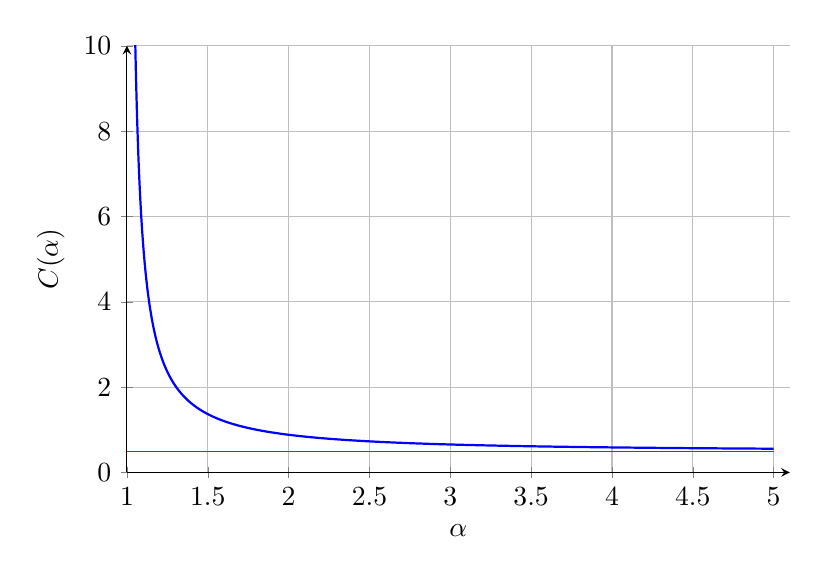
\begin{tikzpicture}
		\begin{axis}[
			axis lines = left,
			xlabel = {$\alpha$},
			ylabel = {$C(\alpha)$},
			xmin=1, xmax=5.1,
			ymin=0, ymax=10, % Clips the peak so the rest of the curve is visible
			grid=major,
			width=10cm,
			height=7cm,
			title={}
			]
			% Paste the coordinates block here
			\addplot[blue, thick, smooth] coordinates {
				(1.0010, 500.3466) (1.0011, 460.1642) (1.0012, 423.2110) (1.0013, 389.2276) (1.0014, 357.9752) (1.0015, 329.2345) (1.0017, 302.8034) (1.0018, 278.4966) (1.0020, 256.1431) (1.0021, 235.5860) (1.0023, 216.6811) (1.0025, 199.2954) (1.0027, 183.3069) (1.0030, 168.6034) (1.0032, 155.0815) (1.0035, 142.6462) (1.0038, 131.2104) (1.0042, 120.6936) (1.0045, 111.0219) (1.0049, 102.1275) (1.0053, 93.9480) (1.0058, 86.4258) (1.0063, 79.5081) (1.0069, 73.1463) (1.0075, 67.2958) (1.0081, 61.9155) (1.0088, 56.9676) (1.0096, 52.4173) (1.0104, 48.2328) (1.0114, 44.3845) (1.0123, 40.8455) (1.0134, 37.5909) (1.0146, 34.5979) (1.0159, 31.8454) (1.0173, 29.3141) (1.0188, 26.9863) (1.0204, 24.8455) (1.0222, 22.8769) (1.0241, 21.0664) (1.0262, 19.4014) (1.0285, 17.8703) (1.0310, 16.4623) (1.0337, 15.1674) (1.0367, 13.9766) (1.0399, 12.8815) (1.0434, 11.8745) (1.0472, 10.9484) (1.0513, 10.0967) (1.0558, 9.3136) (1.0607, 8.5934) (1.0660, 7.9311) (1.0717, 7.3221) (1.0780, 6.7621) (1.0848, 6.2472) (1.0922, 5.7736) (1.1003, 5.3382) (1.1090, 4.9379) (1.1186, 4.5697) (1.1289, 4.2313) (1.1402, 3.9201) (1.1524, 3.6340) (1.1657, 3.3709) (1.1802, 3.1291) (1.1960, 2.9069) (1.2131, 2.7026) (1.2317, 2.5148) (1.2520, 2.3423) (1.2740, 2.1837) (1.2979, 2.0381) (1.3240, 1.9042) (1.3523, 1.7813) (1.3831, 1.6685) (1.4166, 1.5649) (1.4530, 1.4697) (1.4925, 1.3825) (1.5356, 1.3024) (1.5824, 1.2290) (1.6333, 1.1618) (1.6886, 1.1001) (1.7488, 1.0437) (1.8142, 0.9920) (1.8854, 0.9448) (1.9628, 0.9016) (2.0469, 0.8622) (2.1384, 0.8262) (2.2379, 0.7934) (2.3461, 0.7636) (2.4637, 0.7364) (2.5916, 0.7117) (2.7307, 0.6893) (2.8819, 0.6690) (3.0464, 0.6507) (3.2252, 0.6341) (3.4197, 0.6191) (3.6311, 0.6056) (3.8610, 0.5935) (4.1110, 0.5827) (4.3829, 0.5729) (4.6785, 0.5642) (5.0000, 0.5565) 
			};
			\addplot[red] {0.5};
		\end{axis}
	\end{tikzpicture}
	\caption{The blue graph shows $C(\alpha)$ and the red one shows the asymptote at $\frac{1}{2}$.}
	\label{plotOfC(a)}
	\end{figure}
	
	\section*{Figures on convergence}
	\begin{figure}[H]
		\centering
		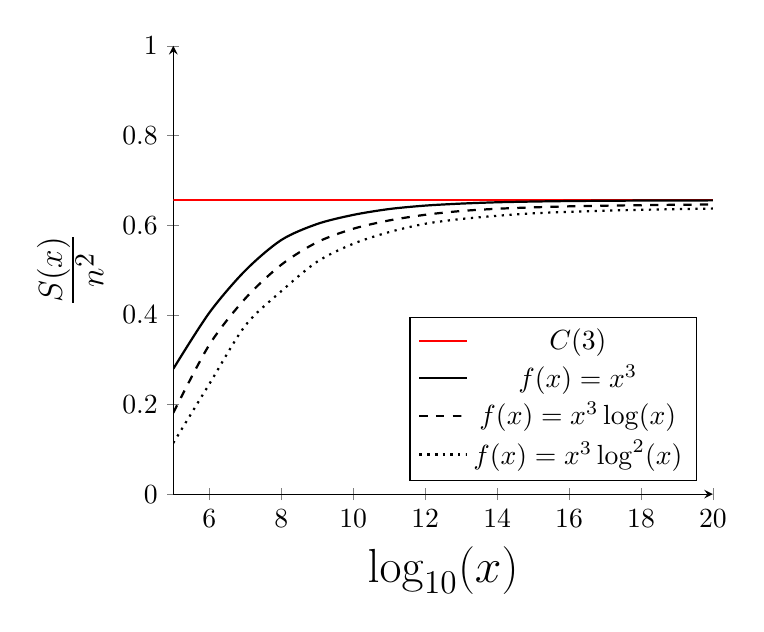
\begin{tikzpicture}
			\begin{axis}
				[
					label style = { font = \LARGE },
					ymode=normal,
					axis lines=left,
					xlabel=$\log_{10}(x)$,
					ylabel=$\frac{S(x)}{n^2}$,
					ymin=0,
					ymax=1,
					legend pos=south east,
				]
				\addplot[red, thick, domain=5:20] {0.655514388573};
				\addlegendentry{$C(3)$}
				\addplot[smooth, thick] table{
					5 	 0.279586
					6 	 0.404537
					7 	 0.498704
					8 	 0.566753
					9 	 0.602608
					10	 0.622818
					11	 0.63592
					12	 0.643569
					13	 0.648045
					14	 0.65099
					15	 0.652635
					16	 0.653749
					17	 0.654374
					18	 0.654807
					19 	 0.655054
					20	 0.655219
				};
				\addlegendentry{$f(x)=x^3$}
				\addplot[smooth, dashed, thick] table{
					5 0.181406
					6 0.333045
					7 0.436385
					8 0.51158
					9 0.562007
					10 0.591895
					11 0.610496
					12 0.623089
					13 0.631517
					14 0.636507
					15 0.639613
					16 0.641916
					17 0.643398
					18 0.64458
					19 0.645429
					20 0.64612
				};
				\addlegendentry{$f(x)=x^3\log(x)$}
				\addplot[smooth, dotted, thick] table{
					5 0.114187
					6 0.245542
					7 0.375879
					8 0.452546
					9 0.518537
					10 0.558425
					11 0.584521
					12 0.603029
					13 0.613707
					14 0.620829
					15 0.626311
					16 0.629712
					17 0.632283
					18 0.634184
					19 0.635672
					20 0.636922	
				};
				\addlegendentry{$f(x)=x^3\log^2(x)$}
			\end{axis}
			
		\end{tikzpicture}
		\caption{Example of how the slowly varying part affects convergence}
		\label{SVeffectsOnConvergence}
	\end{figure}
	
	\begin{figure}[H]
		\centering
		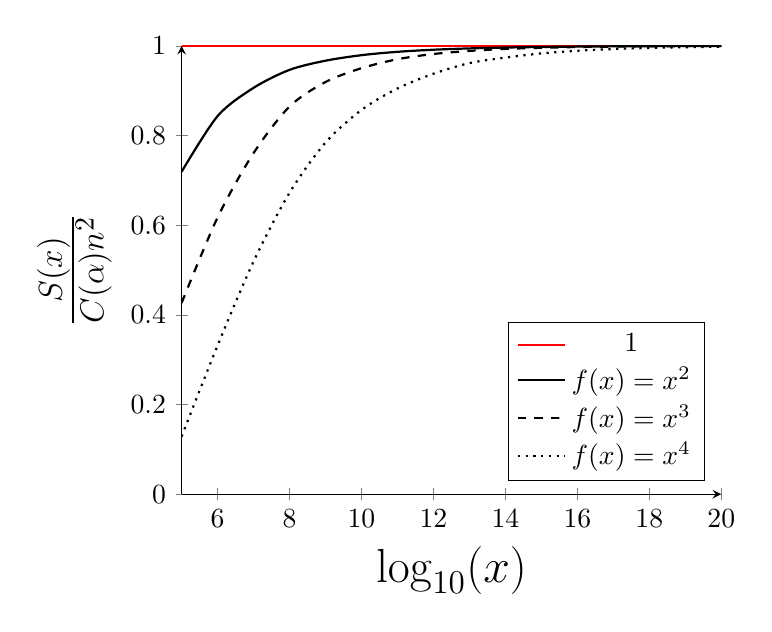
\begin{tikzpicture}
			\begin{axis}
				[
					label style = { font = \LARGE },
					ymode=normal,
					axis lines=left,
					xlabel=$\log_{10}(x)$,
					ylabel=$\frac{S(x)}{C(\alpha)n^2}$,
					ymin=0,
					ymax=1,
					legend pos=south east,
				]
				\addplot[red, thick, domain=5:20] {1};
				\addlegendentry{$1$}
				\addplot[smooth, thick] table{
					5 0.7190649474
					6 0.8432680421
					7 0.9062543204
					8 0.9463711807
					9 0.9668099942
					10 0.9791124528
					11 0.9866137034
					12 0.991276796
					13 0.9942134461
					14 0.9961380048
					15 0.997401421
					16 0.9982504911
					17 0.9988154056
					18 0.999195789
					19 0.9994539063
					20 0.9996293808
				};
				\addlegendentry{$f(x)=x^2$}
				\addplot[smooth, dashed, thick] table{
					5 0.4265139025
					6 0.6171290929
					7 0.7607826902
					8 0.8645927685
					9 0.9192902711
					10 0.9501210208
					11 0.9701083776
					12 0.9817770765
					13 0.9886053019
					14 0.9930979569
					15 0.9956074365
					16 0.9973068653
					17 0.998260315
					18 0.9989208649
					19 0.9992976682
					20 0.999549379
				};
				\addlegendentry{$f(x)=x^3$}
				\addplot[smooth, dotted, thick] table{
					5 0.1286654854
					6 0.3315713285
					7 0.5190241531
					8 0.6722635208
					9 0.7841729099
					10 0.8569712311
					11 0.9049426154
					12 0.9377017748
					13 0.9614184049
					14 0.9736709469
					15 0.9830932284
					16 0.9889955649
					17 0.9928220363
					18 0.99533385
					19 0.9968852143
					20 0.9980551234
				};
				\addlegendentry{$f(x)=x^4$}
			\end{axis}
			
		\end{tikzpicture}
		\caption{Example of how the index affects convergence}
		\label{indexEffectsOnConvergence}
	\end{figure}
	\begin{comment}
	\begin{figure}
		\centering
		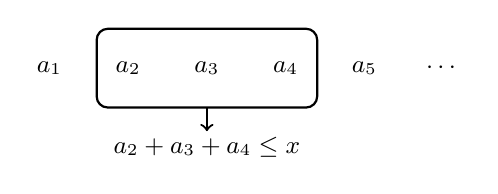
\begin{tikzpicture}[every node/.style={font=\small}]
			
			% sequence elements
			\node (a1) at (0,0)  {$a_1$};
			\node (a2) at (1,0)  {$a_2$};
			\node (a3) at (2,0)  {$a_3$};
			\node (a4) at (3,0)  {$a_4$};
			\node (a5) at (4,0)  {$a_5$};
			\node (dots) at (5,0)  {$\cdots$};
			
			% box around a2, a3, a4 (the consecutive block)
			\draw[rounded corners, thick]
			(0.6,-0.5) rectangle (3.4,0.5);
			
			% label
			\node at (2,-1) {$a_2 + a_3 + a_4\le x$};
			
			% arrow to the sum
			\draw[->, thick] (2,-0.5) -- (2,-0.8);
			
		\end{tikzpicture}
	\end{figure}
	\end{comment}
	
	%$f\in RV_\alpha\Rightarrow f(x)=x^\alpha L(x), L\in SV$
	%\[\forall \lambda\in \mathbb{R}_{>0} \lim_{x\to\infty} \frac{f(\lambda x)}{f(x)}\in \mathbb{R}_{>0}\]
	%\[\forall \lambda\in \mathbb{R}_{>0} \lim_{x\to\infty} \frac{L(\lambda x)}{L(x)}=1\]
	%\[f\in RV\]
	%\[L\in SV\]
	
	\bibliographystyle{plain}
	\bibliography{references}
\end{document}